\documentclass[UTF8]{ctexart}
\usepackage{amsmath}
\usepackage{amssymb}
\usepackage{background}
\usepackage{booktabs}
\usepackage{enumitem}
\usepackage{geometry}
\usepackage{float}
\usepackage{fontspec}
\usepackage{mathptmx} %mathptmx和times结合使得公式使用times new roman字体
\usepackage{tcolorbox}
\usepackage{tikz}
\usepackage{times}
\usepackage{xcolor}
\usetikzlibrary{positioning, arrows.meta, shapes.misc}



\geometry{a5paper, top=0.1cm, left=1cm, right=1cm, bottom=1cm, footskip=0.3cm, marginparsep=0.1cm}
\setCJKmainfont[BoldFont={汉仪文黑-85W},ItalicFont={方正苏新诗柳楷简体}]{汉仪文黑-55W}
\setfontfamily\Issue{Century Schoolbook}
\newCJKfontfamily\TitleFont{思源宋体 CN Heavy}
\newfontfamily\timesnewroman{Times New Roman}
\setmainfont{Times New Roman}
\colorlet{backcolor}{yellow!80!gray!20!} %若只有两页以内,可删去
\pagecolor{backcolor}
\reversemarginpar

\CTEXsetup[format = {\centering\bfseries\large}, beforeskip = 1pt, afterskip = 0pt]{section}

\newcommand\Black[1]{\textcolor[gray]{0.3}{#1}}
\newcommand\Brown[1]{\textcolor[HTML]{998A4E}{#1}}
\newcommand\Emph[1]{\colorbox{red!20!}{\textcolor{red!80!black}{#1}}}
%\newcommand\Correct[1]{\colorbox{green!20}{\textcolor{green!50!black}{#1}}}
\newcommand\Mathemph[1]{\text{\textcolor{green!60!black}{$#1$}}}
\newcommand\Concept[1]{\colorbox{cyan!10!white}{\textcolor{cyan!40!black}{#1}}}
\newcommand\Notes[1]{\textcolor{yellow!50!black}{\small #1}}
\newcommand\Example[1]{\textcolor{cyan!70!black}{\small #1}}
\newcommand\relation[2]{\langle #1,#2 \rangle}
\newcommand\pos[1]{\hspace{0pt} \marginpar{\footnotesize\ttfamily\textcolor{yellow!50!black}{\hfill #1}}}
\newcommand\otherconcept[1]{\textcolor{green!40!black}{\underline{#1}}}

\newcommand\h{\text{\textcolor{blue}{\,$\wedge$\,}}} %合取
\newcommand\x{\text{\textcolor{red!70!black}{\,$\vee$\,}}} %析取
\newcommand\f{\neg} %非
\newcommand\is{\Leftrightarrow\ } %等价
\newcommand\defines{:=}
\newcommand\lcm{\operatorname{lcm}}
\newcommand\N{\text{\textbf{N}}}
\newcommand\Z{\text{\textbf{Z}}}

%这4个信息随“刊号”更新
\newcommand\IssueNumber{11}
\newcommand\Date{2023-11-25}
%\newcommand\Contributer{@金光日}
\newcommand\Subject{离散数学}


\begin{document}
\backgroundsetup{contents=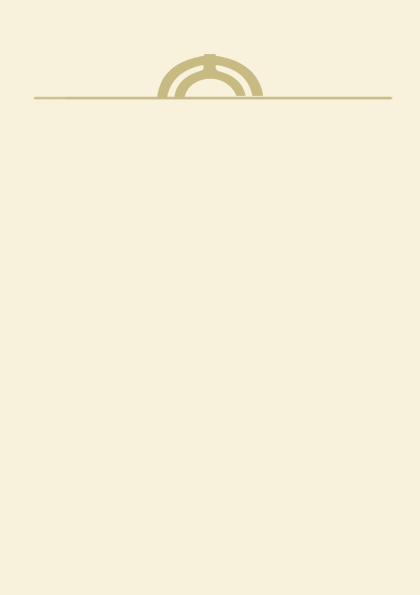
\includegraphics{上半示例.png}, center, scale=1, angle=0, opacity=1}
\BgThispage
\begin{center}
{\scriptsize\Issue \textcolor[HTML]{C8BA83}{WEEKLY TIPS}}

{\Huge\bfseries\TitleFont \Black{知\ 识\ 小\ 料}}

\vspace{-0.1cm}
{\footnotesize \Brown{「电计 2203 班」周常规知识整理共享}}
\end{center}

\vspace{-0.5cm}

\begin{figure}[H]
\hspace{1cm}
\begin{minipage}[t]{0.3\textwidth}
\centering
    \Brown{ISSUE.}

    \vspace{-0.6cm}
    \Huge \Issue\slshape\bfseries\Black{\IssueNumber}
\end{minipage}
\hfill
\begin{minipage}[t]{0.3\textwidth}
\centering
    \Brown{日期:\Date} \\
%\vspace{-0.1cm}
%    \Brown{贡献者:\Contributer} \\
\vspace{-0.1cm}
    \Brown{学科:\Subject} \\
\end{minipage}
\vspace{-0.2cm}
\end{figure}

\begin{flushleft}
\color{cyan!50!black}
本文档给出《离散数学》被跳过的必备数论相关知识,对理解等价关系、划分、群论相关概念有帮助。请读者重点阅读\underline{举例部分},以便理解相关概念。
\end{flushleft}


\section{整除与约数相关}
\begin{description}[itemsep=0pt, parsep=0pt]
    \item[\Concept{整除}] \pos{p185} $a$整除$b$,表示整数$b$除以$a$得到的结果是整数,记为$a|b$;不整除记为$a\nmid b$。

    \Example{举例:$3|12$,$4|-16$,$-3|0$,$5\nmid 21$,$2\nmid -3$。}

    \item[\Concept{因数与倍数}] \pos{p185} 若 $a|b$,则称 $a$ 是 $b$ 的因数(也称\Concept{约数}),$b$ 是 $a$ 的倍数。

    \Example{举例:12 的正因数有 1,2,3,4,6,12,共六个。}

    \item[\Concept{最大公因数}] \pos{p188} 表示两个正整数的公因数中最大的一个,用 $\gcd$ 或 $\mathrm{GCD}$ 表示,记为 $\gcd\{a,b\}$,在不引起混淆的情况下也记为 $(a,b)$。多个数的最大公因数记法类似。其英文为 \underline{g}reatest \underline{c}ommon \underline{d}ivisor。

    \Example{举例:$\gcd\{4,6\}=2$,$\gcd\{8,12\}=4$,$\gcd\{1,3\}=1$。}

    \Notes{思考:对于半群 $\relation{\N ^*}{\odot}$,其中 $a\odot b=\gcd\{a,b\}$,其零元为 1。}

    \item[\Concept{最小公倍数}] \pos{p190} 表示两个正整数的公倍数中最小的一个,用 $\lcm$ 或 $\mathrm{LCM}$ 表示,记为 $\lcm\{a,b\}$,在不引起混淆的情况下也记为 $[a,b]$。多个数的最小公倍数记法类似。其英文为 \underline{l}owest \underline{c}ommon \underline{m}ultiple。

    \Example{举例:$\lcm\{4,6\}=12$,$\lcm\{8,12\}=24$,$\lcm\{1,3\}=3$。}

    \Notes{思考:对于独异点 $\relation{\N ^*}{\otimes}$,其中 $a\otimes b=\lcm\{a,b\}$,其幺元为 1。}
\end{description}

\section{质数相关}
\begin{description}[itemsep=0pt, parsep=0pt]
    \item[\Concept{质数与合数}] \pos{p186} 大于 1 且只能被 1 和它本身整除的数,称为质数(也称\Concept{素数});否则称为合数。由此定义可知,正整数分为质数、合数和 1。

    \Example{举例:2,3,5,7,11,13,17,19,23,29 等是质数,4,6,8,9 等是合数。}

    \item[\Concept{互质}] \pos{p188} 如果两个正整数的最大公因数为 1,则它们互质(也称\Concept{互素})。

    \Example{举例:$\gcd\{25,36\}=1$,因此 25 和 36 互质,但其实它们都是合数。}

    \item[\Concept{欧拉函数$\varphi(m)$}] \pos{p196} 小于或等于 $m$ 且与 $m$ 互质的正整数个数,记为 $\varphi(m)$,称为欧拉函数。

    \Example{举例:$\varphi(6)=2$,因为在 $\{1,2,3,4,5,6\}$ 中,只有 1,5 与 6 互质。}
\end{description}

\newpage
\backgroundsetup{contents=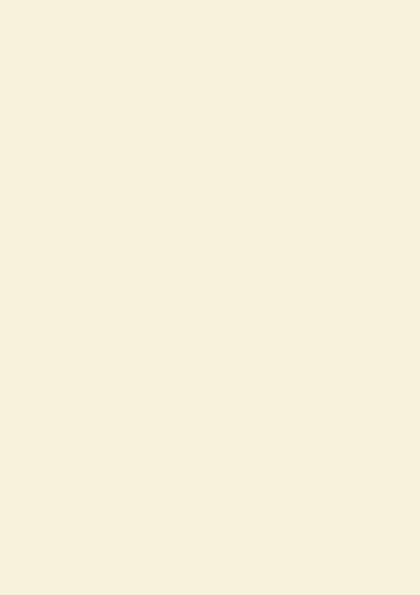
\includegraphics{空白示例.png}, center, scale=1, angle=0, opacity=1}
\BgThispage
\begin{quote}
    \Notes{思考:课本 p266 的定理 13.5.6:若 $\relation{G}{\odot}$ 是 $n$ 阶循环群,则其含有 $\varphi(n)$ 个生成元。例如,$6$ 阶循环群 $\relation{\{e,a,a^2,a^3,a^4,a^5\}}{\odot}$ 中,$a,a^5$ 可成为生成元(因为只有由 $a$ 或 $a^5$ 才可生成集合中的所有元素),共 2 个,即 $\varphi(6)$ 个。}
\end{quote}

\section{余数与同余相关}
\begin{description}[itemsep=0pt, parsep=0pt]
    \item[\Concept{带余数除法}] \pos{p186} 若 $a,b$ 为两个整数,$b\ne 0$,则唯一地存在两个整数 $q,r$,使得 $a=bq+r$(余数 $0\leqslant r < |b|$)。

    \Example{举例:$7\div 3=2\cdots 1$,$7 = 3\times 2 + 1$。}

    \item[\Concept{余数}] \pos{p192} 整数$a$除以正整数$m$ 得到的余数,记为 $a(\bmod m)$ 或 $a\bmod m$。

    \Example{举例:$7(\bmod 3)=1$,$14(\bmod 5)=4$;$-14(\bmod 5)=1$ 因为 $-14=5\times (-3)+1$。}

    \item[\Concept{同余}] \pos{p192} 给定正整数 $m$,若整数 $a$和$b$除以 $m$ 得到的余数相同,则称 $a,b$ 同余,记为 $a\equiv b\pmod m$ 或者 $a\equiv_m b$。

    \Example{举例:$1\equiv 4\pmod 3$,$0\equiv -5\pmod 5$,$-1\not\equiv -2\pmod 3$。}

    \Notes{思考:(1) \otherconcept{$\equiv_m$} 其实也是以符号表示的\otherconcept{等价关系},定义 $\equiv_m \defines \{\relation{x}{y} | x\equiv y\pmod m\}$。}

    \Notes{(2) 同余运算满足下面的式子:
    \begin{equation*}
    \begin{aligned}
        (a\pm b)\pmod m &= (a(\bmod m) \pm b(\bmod m))\pmod m \\
        (a\times b)\pmod m &= (a(\bmod m) \times b(\bmod m))\pmod m
    \end{aligned}
    \end{equation*}
    即对于加、减、乘运算,运算后的模数等于模数的运算。}

    \Notes{(3)若 $x_1\equiv y_1(\bmod m)$,$x_2\equiv y_2(\bmod m)$,则 $x_1+x_2\equiv y_1+y_2 (\bmod m)$。此所谓满足加法的\otherconcept{代换性质}(p244),因此群 $\relation{\Z}{+}$ 的等价关系 $\equiv_m$ 事实上还是\otherconcept{同余关系}。这也正是「同余关系」一词的由来。}

    \item[\Concept{模 $m$ 剩余类}] \pos{p195} 由模 $m$ 余数相同的那些整数构成的集合,称为模 $m$ 剩余类,用 $[r]$ 表示。

    \Notes{形式定义:$[r] \defines \{ i |i\in\Z \h i\equiv r(\bmod m)\}$,其中 $0\leqslant r\leqslant m-1$。}

    \Example{举例:$m=3$,比如模 3 余数都为 0 的那些整数有 $-3,0,3,6,\dots$,我们说 $[0]=\{-3,0,3,6,\dots\}$,再比如 $[1]=\{-2,1,4,7,\dots\}$,$[2]=\{-1,2,5,8,\dots\}$。事实上模 3 剩余类共有 3 个:$[0],[1],[2]$。一般地,模 $m$ 剩余类共有 $m$ 个,它们分别是 $[0],[1],\dots,[m-1]$。}

    \Notes{思考:(1)对于等价关系 $R$,由元素 $x$ 产生的\otherconcept{等价类}一般写成 $[x]_R$。对于“$\equiv_m$”这个用符号表示的等价关系,每一个模 $m$ 剩余系 $[r]$ 就是一个等价类,即 $[r]_{\equiv_m}$。俗话说「物以类聚」——将两个整数聚在同一个模 $m$ 剩余系的条件,就是它们对 $m$ 的模数相同。}

    \Notes{(2)有了等价类,还可以对集合进行\otherconcept{划分},产生\otherconcept{商集},表示所有等价类构成的集合,记为 $A/R$($A$ 是集合,$R$ 是等价关系)。在这里,我们可以用关系“$\equiv_m$”对 $\Z$ 进行划分,产生商集 \otherconcept{$\Z / \equiv_m = \{[0], [1], \dots, [m-1]\}$}。这就相当于把 $\Z$ 分成 $m$ 个「小团体」,每一个「小团体」内的整数对 $m$ 的模数均相同。}
\end{description}


\newpage
\backgroundsetup{contents=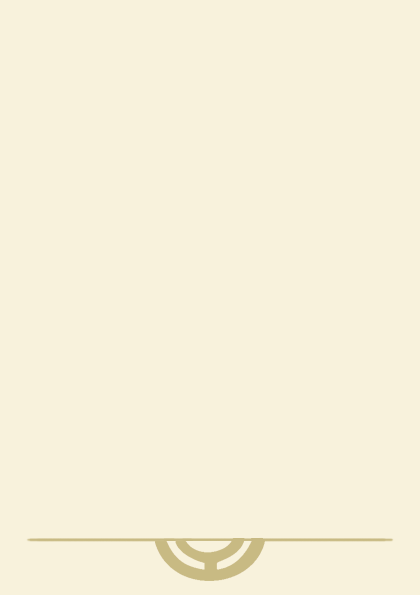
\includegraphics{下半示例.png}, center, scale=1, angle=0, opacity=1}
\BgThispage

\begin{tcolorbox}[colback=cyan!10, colframe=cyan!50!black, boxrule=0.5pt]
\textbf{你了解这些「基数」、「阶数」、「次数」吗?}

\begin{itemize}[itemsep=0pt, parsep=0pt]
    \item 集合 $S$ 的\otherconcept{基数}(也称「势」),表示 $S$ 含有的元素个数,记为 $|S|$。
    \item 运算 $f$ 的\otherconcept{阶}(也称元数),表示 $f$ 所接受的自变量个数。习惯上,用 $\odot$、$\otimes$ 等符号表示的运算是二元运算。
    \item 群 $\relation{G}{\odot}$ 的\otherconcept{阶数},表示集合 $G$ 的元素个数(即 $|G|$)。一般来说有限群才有「阶数」这一说法。
    \item 群中元素 $a$ 的\otherconcept{阶}(也称周期),表示满足 $a^k=e$ 的最小正整数 $k$。如不存在这样的 $k$,则称 $a$ 的阶是无穷的。
    \item 循环群的生成元 $g$ 的\otherconcept{阶},表示满足 $g^k=e$ 的最小正整数 $k$。如不存在这样的 $k$,则称 $g$ 的阶是无穷的。
    \item 置换 $p:X\to X$ 的\otherconcept{阶}表示 $X$ 含有的元素个数(即 $|X|$)。
    \item 轮换 $p:X\to X$ 的\otherconcept{阶}表示其「发生变动」的元素个数。
    
    \Example{举例:$X=\{1,2,3,4,5\}$,$p=\begin{bmatrix} 1&2&3&4&5 \\ 2&4&3&1&5 \end{bmatrix} = (1\ 2\ 4)$ 是 5 阶置换、3 阶轮换。这是因为 $|X|=5$,且「发生变动」的元素有 3 个(即 1,2,4)。}
    
    \item 对称群 $\relation{S_n}{\diamond}$ 的\otherconcept{次数}表示其所依赖的置换集合 $X$ 的基数(即 $|X|$),它的阶数就是 $|S_n|$,即这个群就是 $n$ 次 $n!$ 阶对称群。
        
    \Example{举例:对称群 $\relation{S_3}{\diamond}$,其集合 $S_3$ 有 6 个置换 $\{p_1,p_2,p_3,p_4,p_5,p_6\}$(详见课本 p262 例13.5.1),其复合运算 $\diamond$ 的运算表如课本 p263 页首所示。这些置换 $p_i$ 所依赖的集合是 $X=\{1,2,3\}$,$|X|=3$,因此对称群次数为 3;又因为 $|S_3|=6$,因此对称群阶数为 6。}
\end{itemize}

\end{tcolorbox}

\end{document} 